% Prof. Dr. Ausberto S. Castro Vera
% UENF - CCT - LCMAT - Curso de Ci\^{e}ncia da Computa\c{c}\~{a}o
% Campos, RJ,  2020
% Disciplina: Paradigmas de Linguagens de Programa\c{c}\~{a}o
% Aluno: 



\chapter{ Introdu\c{c}\~{a}o}

Python \'{e} uma poderosa linguagem de programa\c{c}\~{a}o de alto n\'{\i}vel e orientada a objetos, originalmente conceitualizada por Guido van Rossum, no final dos anos 1980, no National Research Institute of Mathematics and Computer Science, Holanda. Python foi a sucessora da linguagem ABC. Python \'{e} uma linguagem  de uso geral, orientada a objetos, com c\'{o}digo bastante leg\'{\i}vel, e com muitas bibliotecas dispon\'{\i}veis e amplamente conhecidas (NumPy, SciPy, Pandas, IPython, Matplotlib, mIPy, ScraPy, etc.)
\begin{quote}
  Python, uma linguagem de script de c\'{o}digo aberto, se tornou a linguagem de ensino introdut\'{o}ria mais popular nas principais universidades americanas - entre elas, Georgia Tech - segundo uma pesquisa recente de Philip Guo, professor assistente de ci\^{e}ncia da computa\c{c}\~{a}o na Universidade de Rochester. Guo decidiu conduzir a pesquisa depois de notar, nos \'{u}ltimos anos, que o Python estava substituindo linguagens como Java como a introdu\c{c}\~{a}o de fato \`{a} classe de programa\c{c}\~{a}o em mais e mais aulas de ci\^{e}ncia da computa\c{c}\~{a}o em universidades de todo o pa\'{\i}s. \cite{Shein2015}
\end{quote}


   \section{Aspectos hist\'{o}ricos da linguagem Python}

A hist\'{o}ria da maioria de linguagens de programa\c{c}\~{a}o n\~{a}o tem uma data fixa, nem um autor \'{u}nico. A sua evolu\c{c}\~{a}o inclui muitos personagens, muitas institui\c{c}\~{o}es e muitas vers\~{o}es.

A seguir, menciona-se alguns aspectos hist\'{o}ricos da linguagem Python, baseados em\cite{Perkovic2016}, \cite{Severance2015} :
\begin{itemize}
  \item O autor principal foi o holand\^{e}s Guido van Rossum, quando trabalhava no CWI ( Centrum Wiskunde \& Informatica), em Amsterd\~{a}, Holanda.
  \item  A linguagem n\~{a}o recebeu esse nome por causada esp\'{e}cie de serpente, mas sim do seriado de com\'{e}dia da BBC \textit{Monty Python's Flying Circus} da qual Rossum \'{e} um f\~{a}.
  \item Python 0.9.0 foi lan\c{c}ado em 1991.  Esta vers\~{a}o incluia manipula\c{c}\~{a}o de exce\c{c}\~{o}es, classes, listas e strings. Tamb\'{e}m foram incl\'{\i}dos alguns aspectos de programa\c{c}\~{a}o funcional: lambda, maps flitros e reduce.

  \item
  \item  Em 1995, Guido continuou se trabalho sobre Python na Corporation for National Research Initiatives (CNRI) em Reston, Virginia, USA.
  \item Python 1.6 foi lan\c{c}ado no CNRI em
  \item  No ano 2000, Guido e a equipe de desenvolvimento principal do Python foram para BeOpen.com para formar a equipe BeOpen PythonLabs.
  \item Python 2.0 foi lan\c{c}ado no ano 2000
  \item Python 3.o foi lan\c{c}ado em dezembro de 2008  \item
  \item
\end{itemize}

Algumas linguagens s\~{a}o consideradas  tradicionais (como mostrado na Fig.\ref{ling1}) e outras s\~{a}o consideradas modernas (ver Fig.\ref{ling2}). Devemos observar aqui, que a inclus\~{a}o de qualquer figura, significa que ela deve ser referenciada em algum lugar do texto
   \begin{figure}[H]
    \begin{center}
        \caption{Logos da Linguagem Python} \label{ling1}
        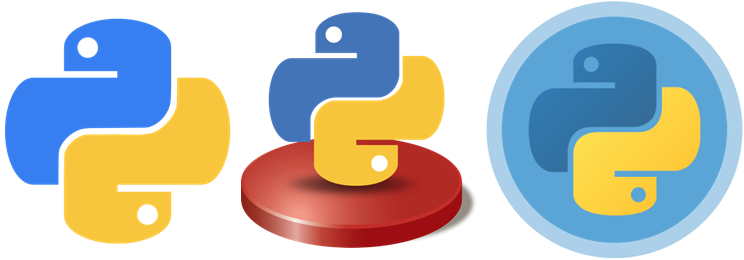
\includegraphics[width=12cm]{Python01.png} \\
        {\tiny \sf Fonte: O autor deste trabalho }
    \end{center}
   \end{figure}

Algumas figuras s\~{a}o criadas o elaboradas pelo mesmo autor, neste caso, deve-se escrever como fonte "O autor", "Os autores", etc. Figuras que incluam imagens de outras fontes deve-se especificar claramente, indicando o link o referencia correspondente, por exemplo, uma imagem que aparece em \cite[p. 93]{Sprankle2012}, \'{e} mostrada na Fig.\ref{afp} e a fonte deve ser indicada na parte inferior da figura.
   \begin{figure}[H]
    \begin{center}
        \caption{Algoritmo, Diagrama de fluxo, e Pseudo-c\'{o}digo} \label{afp}
        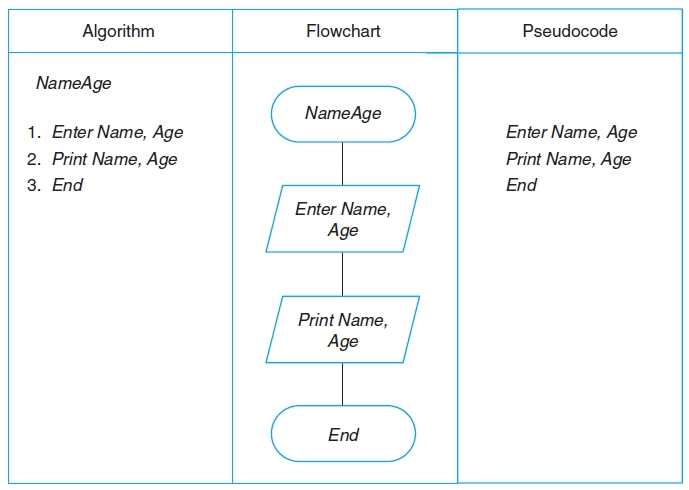
\includegraphics[width=10cm]{afp.jpg} \\
        {\tiny \sf Fonte: \cite[p. 93]{Sprankle2012} }
    \end{center}
   \end{figure}

   \section{\'{A}reas de Aplica\c{c}\~{a}o da Linguagem}
   Esta linguagem \'{e} utilizada e aplicada nas seguintes \'{a}reas: !!!!! As aqui mostradas s\~{a}o exemplos!!!

        \subsection{ Big Data}
        Fazer uma breve descri\c{c}\~{a}o. Pelo menos 3 par\'{a}grafos mencionando exemplos

        \subsection{ Orienta\c{c}\~{a}o a objetos}
        Fazer uma breve descri\c{c}\~{a}o. Pelo menos 3 par\'{a}grafos mencionando exemplos

        \subsection{ outras} 